\documentclass{article}

\def\tags{Public}

\usepackage{amsmath}
\usepackage{amsfonts}
\usepackage{amsthm}
\usepackage{graphicx}
\usepackage[a4paper, total={6in, 8in}]{geometry}

\title{Homework 1}
\date{9 February 2022}
\author{Nicholas Novak (), Yash Karandikar (),\\
Elise Corwin (), Jadriel Delim ()}

\begin{document}
\maketitle

\begin{enumerate}
  \item Consider an improved version of the Vigen\`ere cipher, where instead of
    using multiple shift ciphers, multiple substitution ciphers are used. That
    is, the key consists of $t$ random permutations of the alphabet, and the 
    plaintext characters in positions $i, t + i, 2t + i$, and so on are 
    encrypted using the $i$th permutation. Show how to break this version of 
    the cipher.\\

    First, we make a guess for the length of the key, $l = \vert k\vert$.

    Divide the ciphertext into $l$ different substitution ciphers according to
    the positions of the characters (every $l$th character).

    For example, for a key with a length of $3$, the method would visually
    look like:
    \begin{figure}[h]
      \centering
      \caption{How to split the plaintext with $l = 3$}
      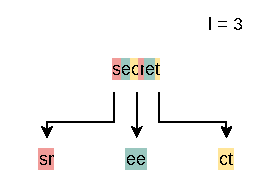
\includegraphics{improved-vigenere-split-diagram.pdf}
    \end{figure}

    From there, we can run frequency analysis on each group, and determine if
    they have a distribution similar to English. From within each group, we can
    get a guess on an individual alphabet for the cipher $k_i$.

    Then, repeat this with multiple values for the guesses on the key length $l$,
    until we find a set of alphabet permutations that seems the most likely.

    From there, the original key $k$ can be found by grouping up all the 
    individual permutations of the individual alphabet guesses $k_i$ in every 
    group.

  \item A Known-Plaintext Attack is an attack scenario where the adversary 
    learns one or more pairs of plaintexts/ciphertexts encrypted under the same
    key. The aim of the adversary is to determine the plaintext that was 
    encrypted in some other ciphertext. Show that the shift, substitution, and 
    Vigen\`ere ciphers are all trivial to break using a known plaintext attack. 
    How much known plaintext is needed to completely recover the key for each
    of the ciphers?\\

    \begin{enumerate}
      \item Show that the shift function is trivial to break

        We have some message $m$, which we know the resulting ciphertext $c$
        for, and which is encrypted with some key $k$.

        As such, for every $i$th character in the message, $m_i$, we encrypt 
        them with $k$ to get the resulting ciphertext $c_i$.
        \[
          m_i + k \pmod{26} = c_i \pmod{26}
        \]

        But, since we know the ciphertext and plaintext, we can take any $i$th
        character from the original message, $m_i$, as well as the
        corresponding ciphertext $c_i$, and we can obtain the key $k$ by
        performing:

        \begin{align*}
          m_i + k \pmod{26} &= c_i \pmod{26}\\
          k \pmod{26} &= c_i - m_i \pmod{26}
        \end{align*}

        And, we can find the key for the entire message, since all other 
        characters share the same key. Thus, one character is enough to find 
        the entire key.
      \item Show that the substitution cipher is trivial to break

        We have some message $m$, and the ciphertext $c$. With each $i$th
        character in the message $m_i$, we can get its individual shift $k_i$ by
        using the same equation as the shift cipher:

        \begin{align*}
          m_i + k_i \pmod{26} &= c_i \pmod{26}\\
          k_i \pmod{26} &= c_i - m_i \pmod{26}
        \end{align*}

        This will give us a list of the individual shifts of each character. The
        key can be found by matching each of these shifts $k_i$ with the original
        character $m_i$.

        Thus, to find the entire alphabet of shifts, we need a message that
        contains every character in the alphabet.
      \item Show that the Vigen\'ere cipher is trivial to break

        We have some message $m$, and the ciphertext $c$. For every $i$th
        character in the message $m_i$, we can get its individual shift $k_i$ by
        applying the function:

        \begin{align*}
          m_i + k_i \pmod{26} &= c_i \pmod{26}\\
          k_i \pmod{26} &= c_i - m_i \pmod{26}
        \end{align*}

        This will give us a repeating pattern of shifts, where the key is the
        longest non-repeating substring. However, it is possible that the key
        could be larger than the message, so to guarantee that we find the
        entire key, we need a message that is at least as long as the key being
        used.
    \end{enumerate}

  \item Assume an attacker knows that A user's password is either
    \verb|abcd| or \verb|bedg|
    \begin{enumerate}
      \item Say the user encrypts her password using the shift cipher, and the 
        attacker sees the resulting ciphertext. Show how the attacker can 
        determine the user’s password, or explain why this is not possible.

        Since the attacker knows the possible plaintexts, and the ciphertext,
        they can use each plaintext and decrypt a shift cipher to get a list of
        the individual shifts for each possible message.

        One of the list of shifts will all be identical, and the other will have
        shifts that are not all the same. Since a shift cipher shifts every
        character by the same amount, the key is the one that was found in the
        message that had identical shifts.

      \item Repeat part (a) for the Vigen\`ere cipher using period 2, using 
        period 3, and using period 4.
    \end{enumerate}
  \item Prove or refute:
    \begin{enumerate}
      \item An encryption scheme with message space $\mathcal{M}$ is perfectly
        secret if and only if for every distribution over the message space 
        $\mathcal{M}$, every $m_0, m_1 \in M$, and every $c \in C$ we have 
        $Pr\left[M = m_0 \mid C = c\right] = Pr\left[M = m_1 \mid C = c\right]$.

      \item An encryption scheme with message space M is perfectly secret if and 
        only if for every probability distribution over $\mathcal{M}$ and every
        $c_0, c_1 \in C$ 
        we have $Pr\left[C = c_0\right] = Pr\left[C = c_1\right]$.
    \end{enumerate}
  \item The first definition we gave in class to define perfect secrecy is as follows
    \begin{enumerate}
      \item Prove that Definition 1 implies Definition 2

        \begin{proof}
          We have some perfectly secret encryption scheme over some message 
          space $\mathcal{M}$, and we generate a pair of messages 
          $m_0, m_1 \in \mathcal{M}$.

          Due to $\mathcal{M}$ being perfectly secret, we have that
          \[
            Pr[\mathcal{M} = m_0] = Pr[\mathcal{M} = m_1]
          \]

          Due to the partition of probabilities rule, we also find that
          $\sum\limits_{i} Pr[m_i] = 1$, i.e.
          \[
            Pr[\mathcal{M} = m_0] + Pr[\mathcal{M} = m_1] = 1
          \]

          Thus, we have
          \begin{align*}
            Pr[\mathcal{M} = m_0] + Pr[\mathcal{M} = m_1] &= 1\\
            Pr[\mathcal{M} = m_1] + Pr[\mathcal{M} = m_1] &= 1\\
            2Pr[\mathcal{M} = m_1] &= 1\\
            Pr[\mathcal{M} = m_1] &= \frac{1}{2}\\
          \end{align*}
        \end{proof}

      \item Prove that Definition 2 implies Definition 1
        
        \begin{proof}
          Generate a pair of messages $m_0, m_1 \in \mathcal{M}$.

          Choose some bit $b \in \left\{0, 1\right\}$, and encrypt some message
          $m_b$ with key $k$. Then, guess some random bit 
          $b' \in \left\{0, 1\right\}$.

          Thus, we have that
          \[
            Pr[\text{PrivK}_{\mathcal{M}, \Pi}^{\text{eav}} = 1] = \frac{1}{2}
          \]

          Due to the partition of probabilities, we have that
          \[
            \sum\limits_i Pr[\mathcal{M} = m_i] =  
            Pr[\text{PrivK}_{\mathcal{M}, \Pi}^{\text{eav}} = 1] + 
            Pr[\text{PrivK}_{\mathcal{M}, \Pi}^{\text{eav}} = 0] = 1
          \]

          Finally, we find that
          \begin{align*}
            Pr[\text{PrivK}_{\mathcal{M}, \Pi}^{\text{eav}} = 1] + 
            Pr[\text{PrivK}_{\mathcal{M}, \Pi}^{\text{eav}} = 0] &= 1\\
            \frac{1}{2} + Pr[\text{PrivK}_{\mathcal{M}, \Pi}^{\text{eav}} = 0] &= 1\\
            Pr[\text{PrivK}_{\mathcal{M}, \Pi}^{\text{eav}} = 0] &= \frac{1}{2}
          \end{align*}

          Substituting this back into the original function, we get that
          \begin{align*}
            Pr[\text{PrivK}_{\mathcal{M}, \Pi}^{\text{eav}} = 1] 
            + \frac{1}{2} &= 1\\
                          &= \frac{1}{2}
          \end{align*}

          Since we find that $Pr[\text{PrivK}_{\mathcal{M}, \Pi}^{\text{eav}} =
          1] = \frac{1}{2} = Pr[\text{PrivK}_{\mathcal{M}, \Pi}^{\text{eav}} =
          0]$, the message space $\mathcal{M}$ must be perfectly secret, due to
          the definition of perfectly secret.
        \end{proof}
    \end{enumerate}
\end{enumerate}

\end{document}
